%%%%%%%%%%%%%%%%%%%%%%%%%%%%%%%%%%%%%%%%%%%%%%%%%%%%%%%%%%%%%%%%
%%                                                            %%
%% aGreekPrimer, Italian translation 2016.12 - 2017           %%
%%                                                            %%
%% From:  Clarence W. Gleason, A Greek Primer                 %%
%%        (1903, New York, American Book Company)             %%
%%                                                            %%
%%        https://archive.org/details/greekprimer00glea       %%
%%                                                            %%
%% Translated by g.p.ciceri <gp.ciceri@gmail.com>             %%
%% ---------------------------------------------------------- %%
%% This translation is Licensed under                         %%
%% Creative Commons Attribution-ShareAlike 4.0 International  %%
%% https://creativecommons.org/licenses/by-sa/4.0/            %%
%%                                                            %%
%%%%%%%%%%%%%%%%%%%%%%%%%%%%%%%%%%%%%%%%%%%%%%%%%%%%%%%%%%%%%%%%

% ᾶῖῶῆῦ  
% ἀἰὐἐὀὠἠ 
% ὰὲὶὸὺὼὴ 
% ἁἱὑὁὡἡῥ
% άέίόύήώΆΉ
% ἂἒὒἲὂὢἢὒἚἊ
% ἃἳὓὃἣὣἓἋἛ
% ἄἔἴὄὔὤἤἌἬ
% ἅἕἵὅὕὥἥἍἭ
% ἆὦἶἦὖἯἏὯἇὧἷἧὗἯἏὯ 

% ᾳῃῳ
% ᾱῑῡ
% ᾀᾐᾠ
% ᾰῐῠ
% ᾂᾒᾢ
% ϊ ϋ
% ᾄᾔᾤ
% ΰ ΐ
% ᾆᾖᾦ
% ᾲῂῲ
% ᾴῄῴ
% ᾷῇῷ
% ᾳῃῳ
% ᾱῑῡ
% ᾰῐῠ

% āēīōū
% ăĕĭŏŭ


\documentclass[nols]{tufte-handout}

%\geometry{showframe} % display margins for debugging page layout

\usepackage{fontspec}
\usepackage{ifxetex}
\setmainfont[Path=./fonts/palatino-linotype/, ItalicFont=palai.ttf, BoldFont=palab.ttf]{pala.ttf}
%\setmainfont[Path=./fonts/GFS_Didot/, ItalicFont=GFSDidotItalic.ttf, BoldFont=GFSDidotBold.ttf]{GFSDidot.ttf}

\newfontfamily\GFSDidotBf[Path=./fonts/GFS_Didot/]{GFSDidotBold.ttf}
\newfontfamily\GFSDidot[Path=./fonts/GFS_Didot/]{GFSDidot.ttf}

\newcommand{\didobf}[1]{{\GFSDidotBf #1}}
\newcommand{\dido}[1]{{\GFSDidot #1}}

\usepackage{lipsum}
\usepackage{url}
\usepackage{longtable}
\usepackage{stackengine}

\usepackage{graphicx} % allow embedded images
  \setkeys{Gin}{width=\linewidth,totalheight=\textheight,keepaspectratio}
  \graphicspath{{graphics/}} % set of paths to search for images
\usepackage{amsmath}  % extended mathematics
\usepackage{booktabs} % book-quality tables
\usepackage{units}    % non-stacked fractions and better unit spacing
\usepackage{multicol} % multiple column layout facilities
\usepackage{lipsum}   % filler text
\usepackage{fancyvrb} % extended verbatim environments
  \fvset{fontsize=\normalsize}% default font size for fancy-verbatim environments

% Standardize command font styles and environments
\newcommand{\doccmd}[1]{\texttt{\textbackslash#1}}% command name -- adds backslash automatically
\newcommand{\docopt}[1]{\ensuremath{\langle}\textrm{\textit{#1}}\ensuremath{\rangle}}% optional command argument
\newcommand{\docarg}[1]{\textrm{\textit{#1}}}% (required) command argument
\newcommand{\docenv}[1]{\textsf{#1}}% environment name
\newcommand{\docpkg}[1]{\texttt{#1}}% package name
\newcommand{\doccls}[1]{\texttt{#1}}% document class name
\newcommand{\docclsopt}[1]{\texttt{#1}}% document class option name
\newenvironment{docspec}{\begin{quote}\noindent}{\end{quote}}% command specification environment

% concetti morfosintattici
\usepackage{xspace} 
\newcommand{\noun}{\textsc{sostantivo}\xspace}
\newcommand{\nouns}{\textsc{sostantivi}\xspace}
\newcommand{\adject}{\textsc{aggettivo}\xspace}
\newcommand{\adjects}{\textsc{aggettivi}\xspace}
\newcommand{\gnumber}{\textsc{numero}\xspace}
\newcommand{\gnumbers}{\textsc{numeri}\xspace}
\newcommand{\gender}{\textsc{genere}\xspace}
\newcommand{\genders}{\textsc{generi}\xspace}
\newcommand{\gcase}{\textsc{caso}\xspace}
\newcommand{\gcases}{\textsc{casi}\xspace}
\newcommand{\tense}{\textsc{tempo}\xspace}
\newcommand{\mood}{\textsc{modo}\xspace}
\newcommand{\gverb}{\textsc{verbo}\xspace}
\newcommand{\gverbs}{\textsc{verbi}\xspace}
\newcommand{\adjective}{\textsc{aggettivo}\xspace}
\newcommand{\nom}{\textsc{nom}\xspace}
\newcommand{\gen}{\textsc{gen}\xspace}
\newcommand{\dat}{\textsc{dat}\xspace}
\newcommand{\acc}{\textsc{acc}\xspace}
\newcommand{\voc}{\textsc{voc}\xspace}
\newcommand{\gexit}{\textsc{uscita}\xspace}
\newcommand{\gexits}{\textsc{uscite}\xspace}
\newcommand{\declinazione}{\textsc{declinazione}\xspace}
\newcommand{\masc}{\textsc{maschile}\xspace}
\newcommand{\femm}{\textsc{femminile}\xspace}
\newcommand{\neut}{\textsc{neutro}\xspace}

\newcommand{\indic}{\textsc{indicativo}\xspace}
\newcommand{\imper}{\textsc{imperativo}\xspace}
\newcommand{\gcong}{\textsc{congiuntivo}\xspace}
\newcommand{\ott}{\textsc{ottativo}\xspace}
\newcommand{\partic}{\textsc{participio}\xspace}
\newcommand{\infin}{\textsc{infinito}\xspace}

\newcommand{\pres}{\textsc{presente}\xspace}
\newcommand{\imperf}{\textsc{imperfetto}\xspace}
\newcommand{\aor}{\textsc{aoristo}\xspace}
\newcommand{\fut}{\textsc{futuro}\xspace}

\newcommand{\sing}{\textsc{singolare}\xspace}
\newcommand{\plur}{\textsc{plurale}\xspace}
\newcommand{\dual}{\textsc{duale}\xspace}


% italianitudini
\renewcommand{\figurename}{Figura}
\renewcommand{\tablename}{Tabella}
\renewcommand{\contentsname}{Indice}

% fix per un qualche problema
\ifxetex
  \newcommand{\textls}[2][5]{%
    \begingroup\addfontfeatures{LetterSpace=#1}#2\endgroup
  }
  \renewcommand{\allcapsspacing}[1]{\textls[15]{#1}}
  \renewcommand{\smallcapsspacing}[1]{\textls[10]{#1}}
  \renewcommand{\allcaps}[1]{\textls[15]{\MakeTextUppercase{#1}}}
  \renewcommand{\smallcaps}[1]{\smallcapsspacing{\scshape\MakeTextLowercase{#1}}}
  \renewcommand{\textsc}[1]{\smallcapsspacing{\textsmallcaps{#1}}}
\fi

\title{A Greek Primer. Introduzione al Greco Antico \newline Lezione IX - Regole di sintassi comuni a Latino e Greco.}

\author[gpciceri]{a cura di Milagathòs: Milo's help to enjoy humanities}

\date{5 Gennajo 2017} % without \date command, current date is supplied


\begin{document}

\maketitle% this prints the handout title, author, and date

\begin{marginfigure}[-3.0cm]
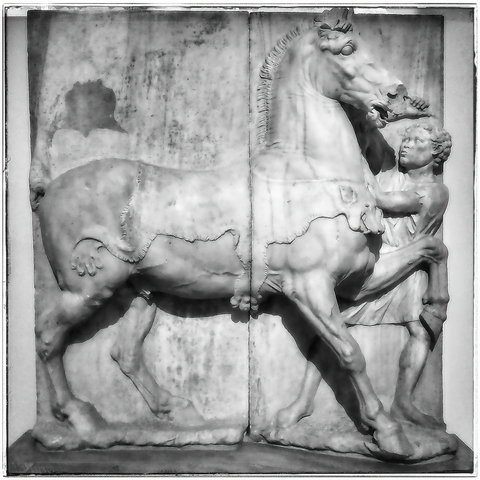
\includegraphics{smallthumb-lesson_I.jpeg}
\setfloatalignment{b}
\end{marginfigure}


\begin{abstract}
\noindent
Queste lezioni si articolano in \textsc{elementi grammaticali}, 
espressi sommariamente, seguiti da \textsc{vocabolari} per il lessico di base 
e da \textsc{frasi da tradurre} dal greco e in greco. 
\
L'approccio è quello del testo-laboratorio di morfosintassi: 
si presenta punto per punto - riprendendone la numerazione - 
l'esposizione di Gleason\cite{gleason1903}.\\
\bigskip
\noindent
Lezione IX: alcune regole di sintassi comuni a Latino e Greco.
\end{abstract}

%\printclassoptions

\newthought{103.} Il soggetto di un verbo finito\sidenote{\textit{verbo finito}: verbo coniugato in un \textit{modo finito}} va in caso nominativo.

\newthought{104. Predicato Nominale.} In un predicato, un nome che significa una stessa persona o cosa del soggetto va nello stesso caso del soggetto, il nominativo. 

\newthought{105. Concordanza dell'Apposizione.} Un nome, usato per descriverne un altro, che si 
riferisce ad una stessa persona o cosa concorda con essa nel caso.

\newthought{106. Concordanza dell'Aggettivo.} L'aggettivo concorda con il nome cui
si riferisce in genere, numero e caso.

\newthought{107. Complemento Oggetto (diretto).} L'oggetto diretto di un verbo transitivo va in caso accusativo.

\newthought{108. Complemento predicativo dell'oggetto.} I verbi che
significano nominare, scegliere, creare, pensare, considerare (e simili),
possono avere un predicato in accusativo in aggiunta al complemento oggetto.

\newthought{109.} L'accusativo viene usato per denotare estensione di tempo (tempo continuato) o di spazio.

\newthought{110. Genitivo di Specificazione.} Un nome usato per definire un altro nome e che non si riferisce alla stessa persona o cosa, va in genitivo.

\newthought{111. Genitivo di Possesso, Soggettivo e Oggettivo.} Il genitivo attributivo può denotare possesso o il soggetto (o l'oggetto) di un'azione o di un sentimento.

\newthought{112. Genitivo Partitivo.} Il genitivo è usato per denotare l'intero insieme, dopo una parola che ne esprime una parte.

\newthought{113. Complemento di Termine o oggetto indiretto.} L'oggetto indiretto di un verbo transitivo va in dativo.

\newthought{114. Dativo e verbi intransitivi.} Il dativo viene usato dopo certi verbi intransitivi che significano servire, credere, piacere, giovare, obbedire (e i loro opposti).

\newthought{115. Dativo di Possesso.} Il dativo è usato dopo \didobf{εἰμί}, \textit{il verbo essere} per indicare il possessore del soggetto della frase.

\newthought{116.} Il dativo è usato con parole che implicano piacere, vicinanza ed approccio.

\newthought{117.} Il dativo è usato dopo molti aggettivi e avverbi, specialmente quelli con significato affine a verbi che reggono il dativo.

\newthought{118. Vocabolario}

\begin{multicols}{2}
    \noindent \hangindent=1em \didobf{βῖκος, ὁ} \textit{vaso, giara}.  \\
    \noindent \hangindent=1em \didobf{βωμός, ὁ} \textit{altare}.  \\
    \noindent \hangindent=1em \didobf{δένδρον, τό} \textit{albero}.  \\
    \noindent \hangindent=1em \didobf{θάλαττα, ἡ} \textit{mare}.  \\
    \noindent \hangindent=1em \didobf{θεά, ἡ} \textit{dea}.  \\
    \noindent \hangindent=1em \didobf{καπηλεῖον, τό} \textit{taverna}.  \\
    \noindent \hangindent=1em \didobf{κόγχη, ἡ} \textit{guscio}.  \\
    \noindent \hangindent=1em \didobf{νἰκε, ἡ} \textit{vittoria}.  \\
    \noindent \hangindent=1em \didobf{οῖνος, ὁ} \textit{vino}.  \\
    \noindent \hangindent=1em \didobf{πέτρᾱ, ἡ} \textit{roccia}.  \\
    \noindent \hangindent=1em \didobf{πλέθρον, τό} \textit{plethrum,} misura di distanza (circa 30 mt.).  \\
    \noindent \hangindent=1em \didobf{στολή, ἡ} \textit{abito}.  \\
    
	\noindent \hangindent=1em \didobf{λαμβάνω}, aor. \didobf{ἔλαβον}, \textit{prendere}. \\ 
	\noindent \hangindent=1em \didobf{πίνω}, aor. \didobf{ἔπιον}, \textit{bere}. \\ 

	\noindent \hangindent=1em \didobf{παρά}, prep. 
	con \gen \textit{da, dal lato di}; 
	con \dat \textit{vicino a, al lato di}; 
	con \acc \textit{a, verso il lato di}.  \\
	
\end{multicols}

\newthought{119. Traduci:}
\textsc{1.}~\dido{ἐδίωξε δέκα πλέθρα.} \quad
\textsc{2.}~\dido{πέντε τῶν οἰκιῶν.} \quad
\textsc{3.}~\dido{τῷ ἀγγέλῳ ἦν υἱός.} \quad
\textsc{4.}~\dido{τήν τῆς βασιλείας χώραν.} \quad
\textsc{5.}~\dido{οἱ ἀνθρώπων δικαίων λόγοι.} \quad
\textsc{6.}~\dido{φοβερῶν μαχῶν.}

\newthought{120.}
\textsc{1.}~\dido{τὸ δὲ παιδίον ἐπιστολὴν ἔπεμψε τῷ ἀδελφῳ.} \quad
\textsc{2.}~\dido{κελεύσει δὲ τὸν ἀδελφὸν πένειν ἐν τῇ κώμῃ.} \quad
\textsc{3.}~\dido{ἐν γὰρ τῇ ὁδῷ ἔλαβον πέντε βίκους μικρούς.} \quad
\textsc{4.}~\dido{καὶ ἤγαγον τοὺς βίκους παρά τὰς σκηνάς.} \quad
\textsc{5.}~\dido{ἐν δὲ τοῖς καπηλείοις οἱ δοῦλοι ἔπιμον οἶνον.} \quad
\textsc{6.}~\dido{ἐπὶ τῇ θαλάττῃ ἦσαν πέτραι καὶ δένδρα μακρά.} \quad
\textsc{7.}~\dido{ἦσαν δὲ καὶ καλαὶ κόγχαι καὶ λίθοι καλοί.} \quad
\textsc{8.}~\dido{ηὖρε δὲω ὁ ἄγγελος παρὰ τῷ βωμῷ στολὰς καὶ ἱμάτια.} \quad
\textsc{9.}~\dido{ἔλιπε τὰς ἁμάξας παρά τῇ θύρᾳ τοῦ ἱεροῦ.} \quad
\textsc{10.}~\dido{διώξομεν γὰρ τὰ θηρία εἰς τὸ πεδίον.}


\newthought{121. Scrivi in Greco:}
\textsc{1.}~Scagliò la (sua) lancia a 150 metri.\quad
\textsc{2.}~Chi mandò una lettera alla regina? \quad
\textsc{3.}~Gli uomini valorosi ottennero la vittoria\sidenote{usa il \dat di possesso 115.}. \quad
\textsc{4.}~Egli lasciò, tu colpisti, io manderò, noi inseguiremo.

\begin{figure*}[!b]
  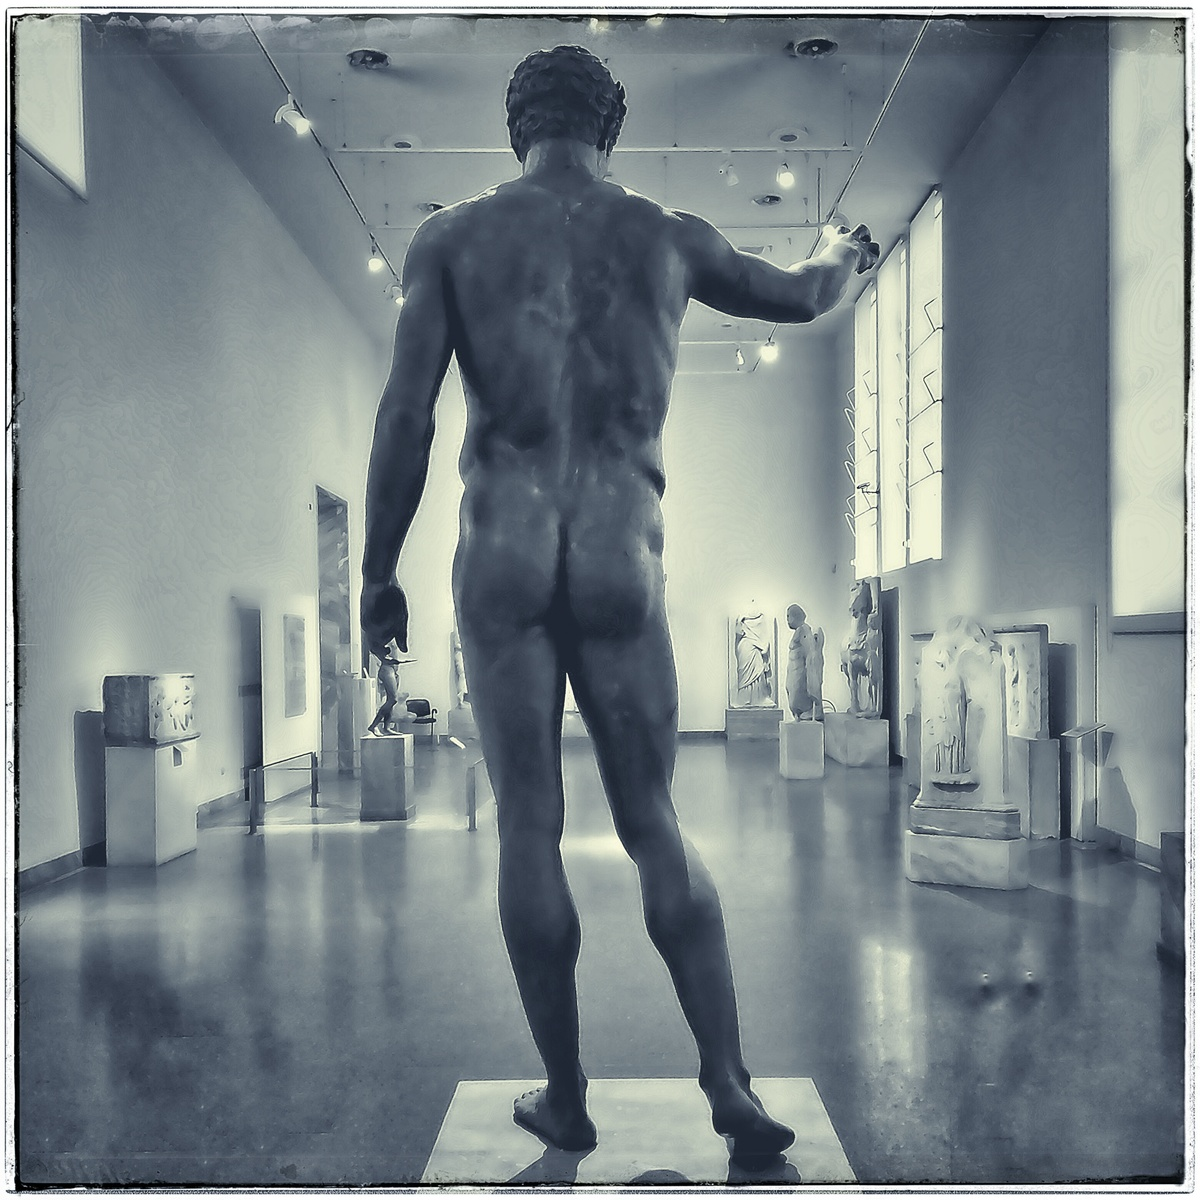
\includegraphics[width=0.9\linewidth]{thumb-lesson_IX.jpeg}
  \caption{Museo Nazionale di Archeologia di Atene}
  \label{fig:textfig}
  %\zsavepos{pos:textfig}
  %\setfloatalignment{b}
\end{figure*}

 

\nobibliography{greekBiblio}
\bibliographystyle{alpha}


\end{document}
